As a new idea, this study introduces a framework for trustless insurance of transport contracts thus replacing the need for centralized intermediation. We propose a mechanism which punishes hostile actors automatically resulting in no conflict resolution required from central entities. The meaning of used abbreviations and function structures in this chapter can be found in the list of symbols appendix A.\par
In our scenario seen at figure \ref{fig:1 main overview}, we assume that the service consumer $A$ wants to send an physical object to the endpoint actor $B$. The third and last actor is the service provider $C$ who will execute the transport contract. Let $A$, $B$ and $C$ all have an Bitcoin public-private key and Bitcoin address which is created with a mapping function from the public key.
% \[CreateKeypair() = \{PubK_i, PrivK_i\}\]
\[CreateKeypair(A) = \{A_{pk}, A_{sk}\}\]
% \[CreateAddress \colon PubK_i \rightarrow Adr_i\]
\[CreateAddress \colon A_{pk} \rightarrow A_{adr}\]
The scenario starts of with $A$ creating a Ricardian contract representing a request for transport, this contract contains $A$ location ($A_{loc}$), $B$ location ($B_{loc}$), $B$ public key ($B_{pk}$), physical object equivalent value ($Ev$) or more and the transport reward ($Tr$).
\[\{A_{loc}, B_{loc}, B_{pk}, Ev, Tr\} \subseteq Rc\]
This contract is accepted by $C$, he will then create and sign an P2SH transaction, denoted by $tx_1$. This transaction contains $Ev$ to be send from $C_{adr}$ to the 2-of-2 multisig P2SH address of $B$ and $C$. Signing a Bitcoin transaction with your private key will include a signature ($C_{sig}$) into the transaction which cannot be decoded back to the private key.

\[CreateAddress \colon \{2, B_{pk}, C_{pk}\} \rightarrow BC_{adr}^{2/2}\]
\[SignTransaction \colon \{Ev, C_{adr}, BC_{adr}^{2/2}, C_{sk}\} \rightarrow tx_1\]

\begin{figure}[h]
\centering
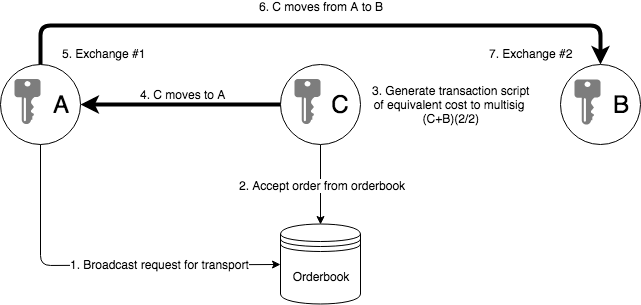
\includegraphics[width=1\textwidth]{images/main.png}
\caption{Overview test scenario}
\label{fig:1 main overview}
\end{figure}

Upon accepting $C$ moves to the physical location of $A$ bringing the signed transaction script $tx_1$. As illustrated with figure \ref{fig:2 first exchange}, upon $C$ arriving at $A$ the asset pickup exchange can take place.

\begin{enumerate}
  \item $C$ innitiates the exchange by giving $A$ the transaction script $tx_1$
  \item $A$ creates and signs a transaction from $A_{adr}$ to the multisig address containing the reward for transporting the physical object.
  \[SignTransaction \colon \{Er, A_{adr}, BC_{adr}^{2/2}, A_{sk}\} \rightarrow tx_2\]
  \item $A$ broadcasts the transport incentive into escrow $\{tx_1, tx_2\}$
  \item $A$ signs and broadcasts the ownership change of the $Rc$ from $A\rightarrow C$
  \item Wait block confirmation containing $\{tx_1, tx_2\}$
  \item Exchange the physical object from $A\rightarrow C$
\end{enumerate}

Before $\{tx_1, tx_2\}$ get broadcasted $A$ or $C$ can individually verify if the signed transactions actually contain what they should.

\begin{figure}[h]
\centering
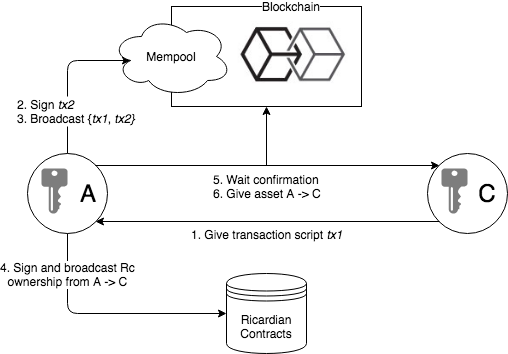
\includegraphics[width=0.8\textwidth]{images/exchange_01.png}
\caption{Asset Pickup Exchange}
\label{fig:2 first exchange}
\end{figure}

 When \textit{C} receives the physical object he is the custodian and will move to the endpoint $B_{loc}$ to claim the reward locked in the escrow. As illustrated with figure \ref{fig:3 drop-off exchange}, upon \textit{C} arriving at $B_{loc}$ the physical object drop-off exchange takes place which consist out of the following steps:

\begin{enumerate}
  \item $B$ signs $tx_3$ containing the equivalent value and transporting reward from $BC_{adr}^{2/2}$ to $C_{adr}$
  \[SignTransaction \colon \{\{tx_1, tx_2\}^{0/2}, BC_{adr}^{2/2}, C_{adr}, B_{sk}\} \rightarrow tx_3\]
  \item $B$ gives the transaction script $tx_3$ to $C$
  \item $C$ signs and broadcasts the ownership change of the $Rc$ from $C\rightarrow B$
  \item Exchange physical object from $C\rightarrow B$
\end{enumerate}

\begin{figure}[h]
\centering
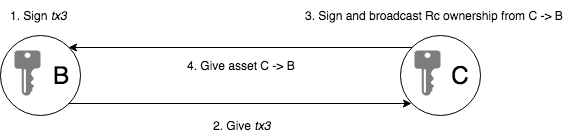
\includegraphics[width=0.8\textwidth]{images/exchange_02.png}
\caption{Asset Dro-poff Exchange}
\label{fig:3 drop-off exchange}
\end{figure}

At the end of the second exchange $C$ now owns $tx_3$ which has been signed by $B$. He can now sign and broadcast the transaction with his own keypair whenever he wants to redeem the funds.

\[SignTransaction \colon \{\{tx_1, tx_2\}^{1/2}, BC_{adr}^{2/2}, C_{adr}, C_{sk}\} \rightarrow tx_3\]
